\chapter{مقدمه} \label{ch:Introduction}

\section{تعریف مسئله و چالش‌ها}
در عصر حاضر، هوش مصنوعی و یادگیری ماشین به یکی از حیاتی‌ترین و پرکاربردترین فناوری‌ها در صنایع مختلف تبدیل شده‌اند. این فناوری‌ها به شرکت‌ها و سازمان‌ها این امکان را می‌دهند تا بهینه‌سازی فرآیندها، پیش‌بینی روندها، و کشف الگوهای پنهان در داده‌ها را با دقت و سرعت بالا انجام دهند. با این حال، بهره‌گیری کامل از قابلیت‌های هوش مصنوعی و یادگیری ماشین نیازمند پیاده‌سازی مؤثر و کارآمد مدل‌های یادگیری ماشین در محیط‌های تولیدی است. در این راستا، مفهومی به نام \lr{MLOps}\footnote{\lr{Machine Learning Operations}} پدید آمده است که به مدیریت، نظارت، و به‌روزرسانی مدل‌های یادگیری ماشین در محیط‌های تولیدی اختصاص دارد.

\lr{MLOps} 
در واقع ترکیبی از مفاهیم \lr{DevOps}\footnote{\lr{Development and Operations}} و \lr{ML}\footnote{\lr{Machine Learning}} است و به هدف ایجاد یک چارچوب یکپارچه برای توسعه، استقرار و مدیریت مدل‌های یادگیری ماشین به کار می‌رود. این مفهوم به شرکت‌ها کمک می‌کند تا چرخه عمر مدل‌های یادگیری ماشین را از مرحله‌ی توسعه تا مرحله‌ی استقرار و نگهداری به صورت مؤثرتری مدیریت کنند. اهمیت \lr{MLOps} به دلیل پیچیدگی‌ها و چالش‌های موجود در پیاده‌سازی مدل‌های یادگیری ماشین در محیط‌های واقعی روز به روز بیشتر می‌شود.

به‌کارگیری مدل‌های یادگیری ماشین در شرکت‌ها به‌طور فزاینده‌ای رو به افزایش است. با این حال، تنها ساختن یک مدل کافی نیست و برای بهره‌برداری کامل از این مدل‌ها، باید آن‌ها را در محیط واقعی به کار برد. به عبارت دیگر، مدل‌های آموزش‌دیده یادگیری ماشین باید به‌صورت عملیاتی در سیستم‌های نرم‌افزاری اصلی شرکت ادغام شوند. این فرآیند که به عنوان استقرار مدل یادگیری ماشین شناخته می‌شود، به سیستم‌های دیگر اجازه می‌دهد تا داده‌ها را به مدل‌ها ارائه کرده و پیش‌بینی‌ها را دریافت کنند که این پیش‌بینی‌ها سپس به سیستم‌های نرم‌افزاری بازگردانده می‌شوند.

با این وجود،  در گزارش \cite{algorithmiaMLState} نشان می‌دهد که بسیاری از شرکت‌ها هنوز راه‌حل مناسبی برای دستیابی به اهداف هوش مصنوعی خود پیدا نکرده‌اند و کاهش فاصله بین ساخت مدل‌های یادگیری ماشین و استقرار عملی آن‌ها همچنان یک چالش اساسی است. ساخت مدل در محیط‌های آزمایشی مانند \lr{Jupyter Notebook} با استقرار مدل در سیستم‌های عملیاتی که ارزش تجاری ایجاد می‌کنند، تفاوت بنیادی دارد. طبق این گزارش، اگرچه بودجه‌های مربوط به هوش مصنوعی در حال افزایش است، تنها ۲۲ درصد از شرکت‌هایی که از یادگیری ماشین استفاده می‌کنند، موفق به استقرار مدل در محیط عملیاتی شده‌اند. این آمار نشان‌دهنده یک فاصله بزرگ در فرآیند پیاده‌سازی می باشد.

علاوه براین، در گزارش \cite{algorithmiaMLState} به بررسی وضعیت یادگیری ماشین در سازمان‌ها پرداخته و از  حدود ۷۵۰ نفر شامل کارشناسان، مدیران پروژه و مدیران اجرایی نظرسنجی راچع به پیاده سازی مدل ها یادگیری ماشین انجام داده است. در این نظرسنجی، نیمی از پاسخ‌دهندگان اظهار داشتند که پیاده‌سازی مدل‌های یادگیری ماشین در شرکت‌هایشان بین یک هفته تا سه ماه طول می‌کشد، در حالی که حدود ۱۸ درصد این مدت را بین سه ماه تا یک سال برآورد کردند (شکل ~\ref{fig: time deploy}). 

\begin{figure}[!t]
	\centering
	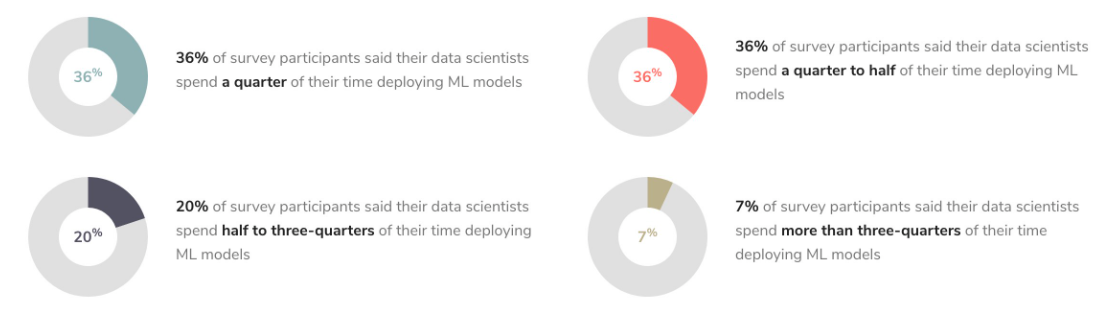
\includegraphics[scale=0.6]{time-deploy.png}
	\caption{زمان استقرار مدل توسط دانشمندان داده}
	\label{fig: time deploy}
\end{figure}


پیاده‌سازی مدل‌های یادگیری ماشین در محیط‌های تولیدی با چالش‌های متعددی همراه است. از جمله این چالش‌ها می‌توان به مدیریت نسخه‌های مختلف مدل‌ها، نظارت بر عملکرد مدل‌ها، اطمینان از تکرارپذیری و قابلیت بازتولید نتایج، و همچنین سازگاری با تغییرات داده‌ها و نیازمندی‌های کسب‌وکار اشاره کرد. \lr{MLOps} با ارائه راهکارهای ساختاریافته و ابزارهای مناسب، به کاهش این چالش‌ها کمک می‌کند و فرآیند استقرار و مدیریت مدل‌های یادگیری ماشین را بهبود می‌بخشد.


در انتها باید اضافه کرد که یکی از دلایل اصلی برای توسعه و استفاده از پلتفرم بومی \lr{MLOps} در ایران، تحریم‌های اعمال شده توسط سرویس‌های بزرگ بین‌المللی مانند
 \lr{Google Vertex AI}،
  \lr{Amazon SageMaker} و \lr{Microsoft Azure ML} است. این تحریم‌ها دسترسی کاربران ایرانی به این سرویس‌ها را محدود کرده و نیاز به یک راه‌حل بومی که بدون وابستگی به سرویس‌های خارجی کار کند را افزایش داده است. با توسعه یک پلتفرم بومی، شرکت‌ها و سازمان‌های ایرانی قادر خواهند بود بدون نگرانی از تحریم‌ها و محدودیت‌ها، به توسعه و استقرار مدل‌های یادگیری ماشین بپردازند. علاوه بر این،‌
  این ارائه‌دهندگان ابری غالبا راه حل قابل قبولی برای شرکت هایی که روی سیستم های نرم افزاری نظارتی یا نرم افزاری هایی با نگرانی های مربوط به حریم خصوصی کاربر کار می کنند نیستند. آن ها به راه حل هایی نیاز دارند که که قابل اجرا روی ابرها و دستگاه های داخلی باشد.
  
  تحقیق حاضر با هدف طراحی و پیاده‌سازی یک پلتفرم \lr{MLOps} به منظور رفع نیازهای موجود در مدیریت مدل‌های یادگیری ماشین و بهبود فرآیندهای توسعه و استقرار آن‌ها انجام شده است. این پلتفرم به گونه‌ای طراحی شده است که قابلیت‌های مختلفی نظیر مدیریت چرخه عمر مدل، نظارت بر عملکرد، به‌روزرسانی خودکار، و تعامل آسان با ابزارهای موجود را فراهم آورد. علاوه بر این، پیاده‌سازی این پلتفرم به صورت ابری انجام می‌شود تا انعطاف‌پذیری و مقیاس‌پذیری بیشتری را به کاربران ارائه دهد.
  
\section{روش تحقیق}

این پایان‌نامه به بررسی و توسعه یک پلتفرم \lr{MLOps} می‌پردازد. روش تحقیق به گونه‌ای طراحی شده‌ است که پاسخگوی سوالات تحقیقاتی زیر باشند:

\begin{enumerate}
	\item 
	چه نیازهایی برای یک پلتفرم \lr{MLOps} مدرن وجود دارد؟
	\item
	چقدر امکان‌پذیر است که یک پلتفرم MLOps با استفاده از ابزارهای متن‌باز موجود به‌صورت ابری طراحی و پیاده‌سازی شود؟
	\item 
	راه‌حل تا چه حد می‌تواند از ارائه‌دهندگان ابر مستقل باشد؟
\end{enumerate}

ابتدا، مسئله به دقت شناسایی و سه سوال تحقیقاتی اصلی مطرح می‌شوند. سپس، مرور جامعی از منابع علمی و مراجع و اسناد اینترنتی برای شناسایی بهترین روش‌ها، ابزارها و چالش‌های موجود در پیاده‌سازی پلتفرم‌های \lr{MLOps} انجام می‌شود. براساس نتایج به‌دست‌آمده از این مرور ادبیات، پلتفرمی با استفاده از ابزارهای متن‌باز ابری طراحی و توسعه داده می‌شود که سهولت استفاده، کارآمدی و قابلیت توسعه را تضمین می‌کند. 


برای طراحی و پیاده‌سازی یک پلتفرم \lr{MLOps} به‌صورت ابری، ابتدا باید نیازمندی‌ها و اهداف پروژه مشخص شوند. سپس، ابزارها و تکنولوژی‌های مناسب انتخاب و معماری سیستم طراحی می‌شود. در نهایت، فرآیندهای توسعه، استقرار و نظارت بر مدل‌ها به‌صورت خودکارسازی شده پیاده‌سازی می‌شوند.

\subsubsection{ابزار متن باز}
برخی از ابزارها و تکنولوژی‌های کلیدی متن باز که برای پیاده‌سازی پلتفرم از آن‌ها استفاده شده است، عبارتند از:
\begin{itemize}
	\item 
	\lr{Kubernetes}:
	 برای مدیریت کانتینرها و فرآیندهای توزیع‌شده استفاده می شود.
	 \item 
	 \lr{Kubeflow}:
	 یک پلتفرم منبع باز برای اجرای جریان‌کاری\footnote{\lr{Workflow}} یادگیری ماشین که بر روی کوبرنتیز اجرا می‌شود.
	 \item 
	 \lr{Jenkins}:
	 یک ابزار اتوماسیون برای پیاده‌سازی فرآیندهای \lr{CI/CD} که امکان خودکارسازی توسعه و استقرار نرم‌افزار را فراهم می‌کند.
	 \item 
	 \lr{Prometheus}:
	 یک سیستم نظارتی و مانیتورینگ که برای جمع‌آوری و تحلیل داده‌های عملکردی استفاده می‌شود.
	 \item
	 \lr{MinIO}:
	 یک سیستم ذخیره‌سازی شی‌گرا که با سازگاری بالا و مقیاس‌پذیری برای مدیریت داده‌های بزرگ طراحی شده است.
	 
\end{itemize}

\subsubsection{طراحی معماری سیستم}

معماری یک پلتفرم \lr{MLOps} شامل لایه‌های مختلفی است که هر کدام نقش خاصی در فرآیند توسعه و استقرار مدل‌ها ایفا می‌کنند. این لایه‌ها عبارتند از:

\begin{itemize}
	\item
لایه داده: شامل ابزارها و فرآیندهای جمع‌آوری، پردازش و ذخیره‌سازی داده‌ها می باشد. این لایه اطمینان حاصل می‌کند که داده‌های مورد نیاز برای آموزش و ارزیابی مدل‌ها به‌صورت بهینه و قابل‌دسترس هستند.
	\item 
لایه مدل‌سازی: شامل ابزارها و محیط‌های توسعه، آموزش و ارزیابی مدل‌ها. این لایه به دانشمندان داده و مهندسان یادگیری ماشین امکان می‌دهد تا مدل‌های خود را به‌سرعت و با دقت بالا توسعه دهند و ارزیابی کنند.
	\item
لایه استقرار: شامل ابزارها و فرآیندهای استقرار و اجرای مدل‌ها در محیط تولید می باشد. این لایه تضمین می‌کند که مدل‌ها به‌صورت پایدار و قابل اعتماد در محیط تولید اجرا شوند.
	\item
لایه نظارت: شامل ابزارها و فرآیندهای نظارتی و مانیتورینگ برای عملکرد مدل‌ها پس از استقرار می باشد. این لایه به تیم‌های عملیاتی امکان می‌دهد تا عملکرد مدل‌ها را به‌صورت مداوم نظارت کنند و در صورت نیاز به‌روزرسانی‌ها و تغییرات لازم را اعمال کنند.
\end{itemize}

\subsubsection{پیاده‌سازی فرآیندهای \lr{CI/CD}}

پیاده‌سازی فرآیندهای \lr{CI/CD} برای مدل‌های یادگیری ماشین به معنای ایجاد یک چرخه تولید و تحویل مداوم است که از توسعه تا نظارت بر مدل‌ها را پوشش می‌دهد. این فرآیند شامل مراحل زیر است:

\begin{itemize}
	\item 
	توسعه و ادغام: کدها و تغییرات جدید به مخزن کد ادغام می‌شوند و تست‌های اتوماتیک اجرا می‌گردند. این مرحله شامل اجرای تست‌های واحد، تست‌های یکپارچگی و تست‌های عملکردی برای اطمینان از صحت و عملکرد کد جدید است.
	\item
	آموزش و ارزیابی: مدل‌ها با استفاده از داده‌های جدید آموزش داده شده و ارزیابی می‌شوند. این مرحله شامل فرآیندهای انتخاب مدل، تنظیم هایپرپارامترها و ارزیابی مدل‌ها برای اطمینان از عملکرد بهینه آنها است.
	\item
	استقرار: مدل‌های تایید شده به محیط تولید منتقل می‌شوند. این مرحله شامل فرآیندهای بسته‌بندی مدل‌ها، پیکربندی محیط تولید و استقرار مدل‌ها به‌صورت خودکار است.
	\item
	نظارت و به‌روزرسانی: عملکرد مدل‌ها نظارت می‌شود و در صورت نیاز به‌روزرسانی‌های لازم اعمال می‌گردد. این مرحله شامل جمع‌آوری داده‌های عملکردی، شناسایی انحرافات و اعمال تغییرات و به‌روزرسانی‌های لازم برای بهبود عملکرد مدل‌ها است.
\end{itemize}


این پلتفرم با استفاده از یک پروژه نمونه یادگیری ماشین پیاده‌سازی و آزمایش می‌شود. نتایج حاصل از این آزمایش‌ها ارزیابی و تحلیل می‌شوند تا میزان پاسخگویی به نیازهای مدرن، امکان‌پذیری پیاده‌سازی با ابزارهای متن‌باز ابری، و میزان استقلال از ارائه‌دهندگان ابر مشخص شود. در نهایت، یافته‌های تحقیق به صورت خلاصه ارائه شده و پیشنهاداتی برای تحقیقات آینده و بهبود پلتفرم ارائه می‌گردد.

\section{ساختار پایان نامه}

در این پایان‌نامه، ساختار به شش بخش اصلی تقسیم می‌شود. در فصل اول، به معرفی و بیان مسائل و چالش‌های تحقیق پرداخته می‌شود. فصل دوم و سوم به بررسی مفاهیم کلیدی \lr{DevOps} و \lr{MLOps}، همراه با مرور پیشینه موضوع و تکنولوژی‌های مرتبط، می‌پردازد. ابزارها و زیرساخت‌های مهم مانند \lr{Docker} و \lr{Kubernetes} به تفصیل معرفی می‌شوند. فصل چهارم به طراحی پلتفرم و سیستم‌های مدیریت مرتبط با \lr{MLOps} اختصاص دارد، که براساس اصول و اجزای معرفی‌شده در فصل‌های قبل، یک پلتفرم \lr{MLOps} طراحی می‌گردد. همچنین، ابزارهای مختلف بررسی و مناسب‌ترین آن‌ها برای طراحی انتخاب می‌شوند. فصل پنجم به پیاده‌سازی معماری طراحی‌شده اختصاص دارد و نتایج حاصل از پیاده‌سازی پلتفرم به نمایش گذاشته می‌شود. برای اعتبارسنجی، دو مسئله یادگیری ماشین بر روی این پلتفرم اجرا می‌شود. نهایتاً، فصل ششم شامل جمع‌بندی، پیشنهادات و نتیجه‌گیری کلی از تحقیق است. 